\subsection{上同伦子与余均衡子的迷向群的比较}

设 H 为一个箭图，G 为一个群胚，\(\varphi\) 与 \(\psi\) 为从 H 到 G 的箭图态射。以 \(\alpha\colon\mathrm{G}\to\mathrm{Coh}(\varphi,\psi)\) 、\(\beta\colon\mathrm{Coh}(\varphi,\psi)\to\mathrm{Coeg}(\varphi,\psi)\) 与 \(\gamma\colon\mathrm{G}\to\mathrm{Coeg}(\varphi,\psi)\) 表示典范群胚态射，以 \(h\) 表示联系 \(\alpha\circ\varphi\) 与 \(\alpha\circ\psi\) 的典范同伦。我们用下面的图表总结这些记号

\pandocbounded{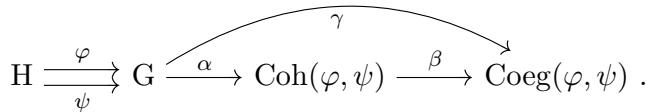
\includegraphics[keepaspectratio]{images/part002_030b7800.jpg}}

在本节（\(n^{o}\)）的余下部分，我们假设偶 \((\varphi,\psi)\) 的框架是一个连通箭图，并固定 G 的一个顶点 \(a_{0}\) 。于是，群胚 \(\mathrm{Coh}(\varphi,\psi)\) 与 \(\mathrm{Coeg}(\varphi,\psi)\) 都是传递的。

以 \(\Gamma\) 表示箭图 \((\mathrm{Som}(\mathrm{G}), \mathrm{Som}(\mathrm{H}), \mathrm{Som}(\varphi), \mathrm{Som}(\psi))\) ，以 \(\widetilde{\Gamma}\) 表示与 \(\Gamma\) 相伴的图，并设 \(\Omega(\widetilde{\Gamma})\) 为有限序列 \((z_1, \ldots, z_n)\) （\(\widetilde{\Gamma}\) 的箭组成的，其中 \(n \geqslant 1\) ）所成的集，这些序列满足：\(z_i\) 的靶是 \(z_{i+1}\) 的起点（若 \(1 \leqslant i < n\) ），且 \(z_n\) 的靶是 \(z_1\) 的起点。在第 1 号中我们构造了一个映射 \(\mathbf{z} \mapsto c(\mathbf{z})\) ，它从集 \(\Omega(\widetilde{\Gamma})\) 映入群 \(\mathrm{Coh}(\varphi, \psi)_{a_0}\) 的共轭类所成的集。

以 \(H \times_{G} H\) 表示 \(H \times H\) 中箭图态射 \(\psi \circ pr_{1}\) 与 \(\varphi \circ pr_{2}\) 的均衡子。其顶点集是 H 的顶点偶 \((a, b)\) （满足 \(\psi(a) = \varphi(b)\) ）所成的集；其箭集是 H 的箭偶 \((f, g)\) （满足 \(\psi(f) = \varphi(g)\) ）所成的集；箭 \((f, g)\) 的起点是顶点 \((o(f), o(g))\) ，其终点是顶点 \((t(f), t(g))\) （参看 II, 第 153 页）。

最后，以 \(\mathrm{Ker}(\varphi, \psi)\) 表示 \(\varphi\) 与 \(\psi\) 的均衡子；回忆（II, 第 165 页, 例 2），这是 H 的子箭图，其顶点 \(a\) 是满足 \(\varphi(a) = \psi(a)\) 的那些顶点，其箭是 \(f \in \mathrm{Fl}(\mathrm{H})\) （满足 \(\varphi(f) = \psi(f)\) ）所成的箭。

命题 4. —— 设 \(\mu\colon\mathrm{H}\times_{\mathrm{G}}\mathrm{H}\to\mathrm{H}\) 为满足 \(\varphi\circ\mu=\varphi\circ\mathrm{pr}_{1}\) 与 \(\psi\circ\mu=\psi\circ\mathrm{pr}_{2}\) 的一个箭图态射。假设：对 H 的每对顶点 \((a,b)\) （满足 \(\varphi(a)=\varphi(b)\) ），存在 H 的一个顶点 \(c\) ，使得 \(\varphi(c)=\psi(b)\) 且 \(a=\mu(b,c)\) 。

  设 \(A_{1}\) 为 \(\mathrm{Ker}(\varphi,\psi)\) 的、与其每个连通分支都相交的顶点集，并设 \(Z_{1}\) 为 \(\Omega(\widetilde{\Gamma})\) 中形如 \(((a,1))\) （其中 \(a\in A_{1}\) ）的元素所成的集。设 \(A_{2}\) 为与 \(H\times_{G}H\) 的每个连通分支都相交的 \(H\times_{G}H\) 的顶点集，并设 \(Z_{2}\) 为形如 \(((a,1),(b,1),(\mu(a,b),-1))\) （其中 \((a,b)\) 取遍 \(A_{2}\) ）的三元组所成的集。

那么，\(\Omega(\widetilde{\Gamma})\) 是 \(\Omega(\widetilde{\Gamma})\) 中包含 \(Z_1 \cup Z_2\) 的最小正规子集。特别地，共轭类 \(c(\mathbf{z})\) （在 \(\mathrm{Coh}(\varphi, \psi)_{a_0}\) 中，其中 \(\mathbf{z}\) 取遍 \(Z_1 \cup Z_2\) ）生成典范同态 \(\beta_{a_0}\) （从 \(\mathrm{Coh}(\varphi, \psi)_{a_0}\) 到 \(\mathrm{Coeg}(\varphi, \psi)_{\beta(a_0)}\) ）的核。

以 \(Z_{1}^{\prime}\) 、\(Z_{2}^{\prime}\) 与 \(Z^{\prime}\) 分别表示 \(\Omega(\widetilde{\Gamma})\) 中包含 \(Z_{1}\) 、\(Z_{2}\) 与 \(Z_{1} \cup Z_{2}\) 的最小正规子集（II, 第 197 页, 定义 1）。目标是证明 \(Z^{\prime}\) 等于 \(\Omega(\widetilde{\Gamma})\) 。由 II, 第 197 页的命题 1 的推论 1（II, 第 199 页），命题的后一断言将由此得出。

引理 1. —— a) 对每个顶点 \(a\) （\(\operatorname{Ker}(\varphi, \psi)\) 的），\(((a, 1))\) 属于 \(Z_1'\) 。

\begin{enumerate}
\def\labelenumi{\alph{enumi})}
\setcounter{enumi}{1}
\item
  对每个顶点 \((a,b)\) （\(\mathrm{H}\times_{\mathrm{G}}\mathrm{H}\) 的），\(((a,1),(b,1),(\mu(a,b),-1))\) 属于 \(\mathbf{Z}_2^{\prime}\) 。
\item
  设 \(A_{1}^{\prime}\) 为顶点 \(a\) （\(\operatorname{Ker}(\varphi,\psi)\) 的，使 \(((a,1))\) 属于 \(Z_{1}^{\prime}\) ）所成的集。我们有 \(A_{1}\subset A_{1}^{\prime}\) （根据 \(Z_{1}^{\prime}\) 的定义）。设 \(f\) 为 \(\operatorname{Ker}(\varphi,\psi)\) 的一条箭，\(a\) 为其起点，\(b\) 为其靶。把正规子集定义中的性质 (iv)（II, 第 197 页, 定义 1）应用于序列 \(((f,1))\) ，便得 \(a\in A_{1}^{\prime}\) 等价于 \(b\in A_{1}^{\prime}\) 。由于 \(A_{1}\) 与 \(\operatorname{Ker}(\varphi,\psi)\) 的每个连通分支相交，我们有 \(A_{1}^{\prime}=\operatorname{Som}(\operatorname{Ker}(\varphi,\psi))\) ，此即所要证明的。
\item
  设 \(A_{2}^{\prime}\) 为顶点 \((a,b)\) （\(H \times_{G} H\) 的，使三元组 \(((a,1),(b,1),(\mu(a,b),-1))\) 属于 \(Z_{2}^{\prime}\) ）所成的集。根据假设，有 \(A_{2} \subset A_{2}^{\prime}\) 。由于 \(A_{2}\) 与 \(H \times_{G} H\) 的每个连通分支相交，只需证明：若存在一条箭 \((f,f^{\prime})\) ，连接顶点 \((a', b')\) 与顶点 \((a, b)\) ，则 \((a, b)\) 属于 \(A_2'\) 当且仅当 \((a', b')\) 亦然。
\end{enumerate}

令 \(f'' = \mu(f, f')\) ；它是一条连接 \(\mu(a', b')\) 与 \(\mu(a, b)\) 的箭，且有 \(\varphi(f'') = \varphi(f)\) 与 \(\psi(f'') = \psi(f')\) 。把 \(\Omega(\widetilde{\Gamma})\) 的正规子集定义中的条件 (iv)（同前）应用于序列 \(((f, 1), (f', 1), (f'', -1))\) ，可知下列两个条件

\begin{enumerate}
\def\labelenumi{(\roman{enumi})}
\item
  三元组 \(((a,1),(b,1),(\mu (a,b), - 1))\) 属于 \(Z^{\prime}\) ；
\item
  三元组 \(((a',1),(b',1),(\mu(a',b'),-1))\) 属于 \(Z'\) 是等价的。这表明 \((a,b)\) 属于 \(A_{2}'\) 当且仅当 \((a',b')\) 属于 \(A_{2}'\) ，引理证明完毕。
\end{enumerate}

我们现在对整数 \(n \geqslant 1\) 作归纳来证明：每个元素 \(((a_1, \varepsilon_1), (a_2, \varepsilon_2), \ldots, (a_n, \varepsilon_n))\) （\(\Omega(\widetilde{\Gamma})\) 的）都属于 \(Z'\) 。

\casehead{\(n = 1\) 的情形}

设 \(((a,\varepsilon))\) 为 \(\Omega(\tilde{\Gamma})\) 的一个长度为 1 的元素。我们有 \(\varphi(a)=\psi(a)\) ，从而 \(((a,1))\in\mathbb{Z}'\)。由引理 1，正规子集定义中的条件 (ii) 进而蕴含 \(((a,-1))\) 属于 \(Z'\) 。

\casehead{\(n \geqslant 2\) 的情形}

根据正规子集的条件 (ii)，只需处理 \(\varepsilon_{2}=1\) 的情形。假设 \(\varepsilon_{1}=1\) ；那么 \((a_{1},a_{2})\) 是 H \(\times_{G}H\) 的一个顶点；令 \(a=\mu(a_{1},a_{2})\) ；由引理 1，三元组 \(((a_{1},1),(a_{2},1),(a,-1))\) 因此属于 \(Z'\)。在 \(\varepsilon_{1}=-1\) 的情形，我们有 \(\varphi(a_{1})=\varphi(a_{2})\) ；因此可以选取 H 的一个顶点 \(a\) ，使得 \(\mu(a_{2},a)=a_{1}\) ，且三元组 \(((a_{2},1),(a,1),(a_{1},-1))\) 属于 \(Z'\) ，于是根据正规子集定义中的条件 (ii)，三元组 \(((a_{1},-1),(a_{2},1),(a,1))\) 也属于 \(Z'\)。

于是，\(((a,\varepsilon_1),(a_3,\varepsilon_3),\ldots ,(a_n,\varepsilon_n))\) 属于 \(\Omega (\widetilde{\Gamma})\) 且长度为 \(n - 1\)。由归纳法，这是 \(\mathbf{Z}'\) 的一个元素。利用正规子集定义中的条件 (i)、(ii) 与 (iii)，我们相继推出下列元素

\[
\begin{array}{c} ((a _ {1}, \varepsilon_ {1}), (a _ {2}, 1), (a, - \varepsilon_ {1}), (a, \varepsilon_ {1}), (a _ {3}, \varepsilon_ {3}), \ldots , (a _ {n}, \varepsilon_ {n})), \\ ((a, - \varepsilon_ {1}), (a, \varepsilon_ {1}), (a _ {3}, \varepsilon_ {3}), \ldots , (a _ {n}, \varepsilon_ {n}), (a _ {1}, \varepsilon_ {1}), (a _ {2}, 1)), \\ ((a _ {3}, \varepsilon_ {3}), \ldots , (a _ {n}, \varepsilon_ {n}), (a _ {1}, \varepsilon_ {1}), (a _ {2}, 1)), \\ ((a _ {1}, \varepsilon_ {1}), (a _ {2}, 1), (a _ {3}, \varepsilon_ {3}), \ldots , (a _ {n}, \varepsilon_ {n})) \end{array}
\]

都属于 Z'。命题证明完毕。

推论. —— a) 采用命题 4 的记号，进一步假设从 Som(H) 映入 Som(G) × Som(G) 的映射 (Som(φ), Som(ψ)) 是单射的，且其像是 Som(G) 上一个等价关系的图。那么，对 H \(\times_{G}\) H 的每个顶点 (a, b)，存在唯一的 H 的顶点 \(c_{a,b}\) ，使得 \(\varphi(c_{a,b}) = \varphi(a)\) 且 \(\psi(c_{a,b}) = \psi(b)\) 。

\begin{enumerate}
\def\labelenumi{\alph{enumi})}
\setcounter{enumi}{1}
\tightlist
\item
  进一步假设：对每条箭 \((f, f')\) （H \(\times_{G}\) H 的），存在 H 的一条箭 \(f''\) ，使得 \(\varphi(f'') = \varphi(f)\) 且 \(\psi(f'') = \psi(f')\) 。
\end{enumerate}

设 A 为与 H \(\times_{G}\) H 的每个连通分支都相交的顶点集。那么，态射 \(\beta_{a_{0}}\) 的核是 \(\mathrm{Coh}(\varphi,\psi)_{a_{0}}\) 中包含共轭类 \(c((a,1),(b,1),(c_{a,b},-1))\) （对 \((a,b)\in\mathrm{A}\) ）的最小正规子群。

设 R 为 \(\operatorname{Som}(\mathrm{G})\) 上以映射 \((\operatorname{Som}(\varphi),\operatorname{Som}(\psi))\) 的像为图的等价关系。设 \((a,b)\) 为 \(H\times_{G}H\) 的一个顶点。于是有 \(\operatorname{R}\{\varphi(a),\psi(a)\}\) 与 \(\operatorname{R}\{\varphi(b),\psi(b)\}\) ，从而 \(\operatorname{R}\{\varphi(a),\psi(b)\}\) （因为 \(\psi(a)=\varphi(b)\) ）。因此，存在唯一的 H 的顶点 \(c\) ，使得 \(\varphi(c)=\varphi(a)\) 且 \(\psi(c)=\psi(b)\) ；把它记作 \(\mu(a,b)\) 。

对每条箭 \((f, f')\) （\(H\times_{G}H\) 的），选取 H 的一条箭 \(f''\) ，使得 \(\varphi(f'') = \varphi(f)\) 且 \(\psi(f'') = \psi(f')\) ，并把它记作 \(\mu(f, f')\) 。

我们就这样定义了一个箭图态射 \(\mu\colon\mathrm{H}\times_{\mathrm{G}}\mathrm{H}\to\mathrm{H}\) ，满足 \(\varphi\circ\mu=\varphi\circ\mathrm{pr}_{1}\) 与 \(\psi\circ\mu=\psi\circ\mathrm{pr}_{2}\) 。

设 \((a,b)\) 为满足 \(\varphi(a)=\varphi(b)\) 的一对 H 的顶点。我们有 \(\mathrm{R}\{\varphi(a),\psi(a)\}\) 与 \(\mathrm{R}\{\varphi(b),\psi(b)\}\) ，因此 \(\mathrm{R}\{\psi(b),\psi(a)\}\) 。从而存在唯一的 H 的顶点 \(c\) ，使得 \(\varphi(c)=\psi(b)\) 且 \(\psi(c)=\psi(a)\) 。顶点 \(\mu(b,c)\) 满足 \(\varphi(\mu(b,c))=\varphi(b)=\varphi(a)\) 与 \(\psi(\mu(b,c))=\psi(c)=\psi(a)\) 。 我们因此有 \(\mu(b,c)=a\) ，因为映射 \((\operatorname{Som}(\varphi),\operatorname{Som}(\psi))\) （从 \(\operatorname{Som}(\operatorname{H})\) 映入 \(\operatorname{Som}(\operatorname{G})\times\operatorname{Som}(\operatorname{G})\) ）是单射的。

设 \(A_{1}\) 为 \(\operatorname{Ker}(\varphi,\psi)\) 的顶点集，并设 \(Z_{1}\) 为 \(\Omega(\widetilde{\Gamma})\) 中形如 \(((a,1))\) （对 \(a\in A_{1}\) ）的元素所成的集。令 \(A_{2}=A\) ，并设 \(Z_{2}\) 为形如 \(((a,1),(b,1),(\mu(a,b),-1))\) 的元素（\(\Omega(\widetilde{\Gamma})\) 的，对 \((a,b)\in A_{2}\) ）所成的集。以 \(\widetilde{Z}\) （相应地 \(\widetilde{Z}_{1}\) ，或 \(\widetilde{Z}_{2}\)）表示 \(\Omega(\widetilde{\Gamma})\) 中包含 \(Z_{1}\cup Z_{2}\) （相应地 \(Z_{1}\) ，或 \(Z_{2}\)）的最小正规子集。

设 \(a \in \mathrm{A}_1\) 。我们有 \(\varphi(a) = \psi(a)\) ；令 \(x = \varphi(a)\)。顶点 \(a\) 是满足 \(\varphi(a) = \psi(a) = x\) 的 H 的唯一顶点。特别地，我们有 \(\mu(a, a) = a\)。因此三元组 \(((a, 1), (a, 1), (a, -1))\) 属于 \(\mathbf{Z}_2\)。进而由正规子集定义中的条件 (i) 与 (iii) 得出 \(((a, 1))\) 属于 \(\widetilde{\mathbf{Z}}_2\)。从而我们有 \(\mathbf{Z}_1 \subset \widetilde{\mathbf{Z}}_2\) ，于是 \(\widetilde{\mathbf{Z}} = \widetilde{\mathbf{Z}}_2\) 。

由命题 4，\(\Omega(\tilde{\Gamma})\) 是 \(\Omega(\tilde{\Gamma})\) 中包含 \(Z_{2}\) 的最小正规子集，且 \(\beta_{a_{0}}\) 的核是 \(\mathrm{Coh}(\varphi,\psi)_{a_{0}}\) 中包含共轭类 \(c(\mathbf{z})\) （对 \(\mathbf{z}\in Z_{2}\) ）的最小正规子群。推论得证。

例. —— 设 X 与 R 为拓扑空间，o 与 t 为从 R 到 X 的连续映射，C 为偶 \((f,g)\in\mathrm{R}^{2}\) （满足 \(t(f)=o(g)\) ）所成的集，m 为使箭图 \((\mathrm{X},\mathrm{R},o,t)\) 成为一个群胚的从 C 到 R 的连续映射；进一步假设从 R 到 R 的映射 \(f\mapsto f^{-1}\) 是连续的。若令 \(\mathrm{H}=\varpi(\mathrm{R})\) 、\(\mathrm{G}=\varpi(\mathrm{X})\) 、\(\varphi=\varpi(o)\) 、\(\psi=\varpi(t)\) 与 \(\mu=\varpi(m)\) ，则命题的假设得到满足。

进一步假设 R 是 X 上一个等价关系的图，其中映射 o 与 t 由 \(X \times X\) 到 X 的投影通过取子空间导出。于是推论的假设得到满足。

注记. —— *更一般地，当 (G, H, \(\varphi\) , \(\psi\) , \(\mu\) ) 是一个“群胚的群胚”时，命题的假设得到满足。这意味着 G 与 H 都是群胚，\(\varphi\) 与 \(\psi\) 是从 H 到 G 的群胚态射，使四元组 (G, H, \(\varphi\) , \(\psi\) ) 成为一个“群胚箭图”；最后，\(\mu\) 是这个“箭图”中由一个群胚态射 H \(\times_{\mathrm{G}}\) H → H 给出的合成法则，它满足表达该法则的结合性以及每条“箭”皆可逆的一定数目的性质。读者还会注意到，本书中所研究的基本群胚的应用全都属于这种情形。

